\section{Introducción}
Esta sección se enfocará a la parte de transmisión de información y que tipo de operaciones lógicas matemáticas ocurren para que un cerebro pueda realizar cómputos, específicamente se detallará la mecánica de los disparos de las neuronas, siendo estos una de las características más relevantes a la hora de modelar las redes neuronales artificiales. Si en algún momento de su vida han visto temas relacionados con compuertas digitales, arquitectura de computadoras, diseño electrónico digital, les será más fácil abstraer el concepto, pues nosotros vamos a ver los procesos de paso de información a través de compuertas pero en un sistema biológico (de la naturaleza). 

Notemos primeramente un impulso nervioso, recordemos que esté es una onda que avanza desde el cono axónico de la neurona hasta la neurona postsináptica. Esta onda electroquímica ocurre dada la diferencia de potencial entre la parte interna y externa de neurona, está diferencia se da a consecuencia de las distintas concentraciones de iones en ambos lados de la membrana plasmática. Los estados en la membrana plasmática (del axón) se pueden diferenciar en, potenciales neuronales:

\begin{itemize}
\item \textbf{Potencial de reposo:} Es la diferencia de cargas en la membrana y está polarizada a -70mV. Es positiva por fuera (Na+ ) y negativa por dentro por Cl- y proteínas- y no transmite señal. 
\item \textbf{Potencial de acción o membrana:} Un estímulo umbral de 55mV, despolariza la membrana y abre los canales del Na+ y K+ y avanza la señal nerviosa, es un cambio muy rápido en la polaridad de la membrana de negativo a positivo y vuelta a negativo.
\end{itemize}

%(Insertar esquema) 
\begin{figure}[h]
 \centering
 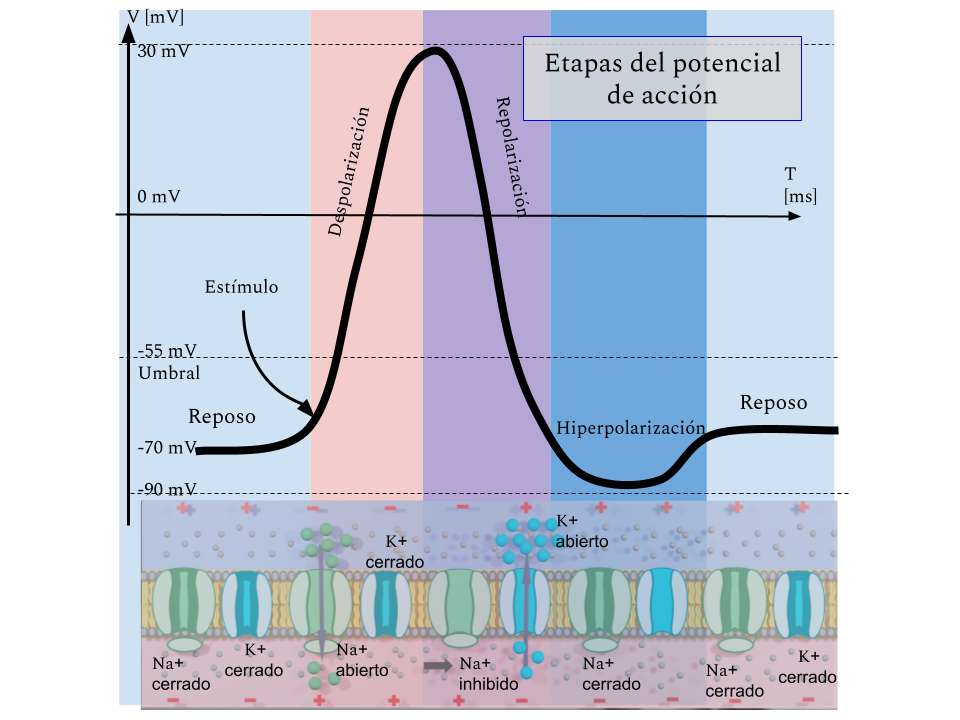
\includegraphics[scale=0.5]{../Figuras/Grafica.png}
 \caption{Representación gráfica de la respuesta de los canales ionicos de sódio (Na+ en verde) y potasio (K+ en azul) ante un estímulo de voltaje, dando como resultado un potencial de acción que viajará a lo largo de todo el axón.}
 \label{fig:graficaP}
\end{figure}

Retomando la sinapsis eléctrica, donde participan los canales iónicos y las entradas de la neuronas (dendritas) están siendo alteradas poco a poco, hasta que ocurre la suficiente carga (diferencia de potencial) en sus dendritas y en el cuerpo de la neurona, para que desde el cono axónico se de un disparo o potencial de acción (spike), transmitiendo la información gracias a la apertura y cierre de ciertos canales de iones cargados. Este cambio brusco de la diferencia de potencial , se nota en forma de un pulso eléctrico (ver \ref{graficaP}),  para saber más a detalle qué está ocurriendo en está rápida elevación en la diferencia de potencial, se contará de dónde salió este modelo y por qué toma la forma que tiene. 

Los primeros científicos que estudiaron el potencial de acción y dieron un modelo (de la unión sináptica eléctrica)  fueron Alan Lloyd Hodgkin y Andrew Fielding Huxley, 
obteniendo un modelo matemático, que intenta explicar qué es lo que estaba pasando en las neuronas. Ellos trabajaron con un calamar gigante (que puede medir hasta 4 metros de largo) dado su gran tamaño, tiene un axón también bastante gigantesco, que recorre casi la mitad del cuerpo del calamar y su grosor es de medio milímetro, considerando el tamaño estándar de una axón de una neurona ( 1-20 um). El axón del calamar gigante es tan grande que les permitió introducir dispositivos para medir el voltaje, es decir, la diferencia de potencial entre, el interior de la neurona y la parte de afuera, el ambiente externo de la neurona. Con estás mediciones experimentales que lograron obtener (1939), se pudo determinar qué pasaba con las cargas eléctricas tanto en el interior como en el exterior y así estudiar cómo se lograba la transferencia de electricidad cuando disparaba este pulso. 
 Se dan cuenta que podían modelar este comportamiento como un circuito eléctrico donde están corriendo estas corrientes, si bien aún no sabían todavía cuál era exactamente el mecanismo biológico por detrás, si observaron que había dos elementos protagónicos que serían el sodio y el potasio.
 Notaron que estos existen en diferentes concentraciones, en la parte de afuera y en la parte de adentro de las neuronas. Con esto nosotros podemos aprender también el por qué es importante consumir algo de sal y nunca estar bajos de potasio, pues estos dos elementos son indispensables para que las neuronas puedan transmitir sus señales. 

\section{Membrana y canal}

Hodgkin y Huxley se dedicaron a estudiar qué pasaba con las concentraciones de estos iones (sodio y potasio) en la parte de afuera o en la parte de adentro cuando empezaban a fluir las corrientes. El sistema parecía una especie de circuito eléctrico, se lo imaginaron como una especie de membrana porosa (lo cual es bastante cercano a lo que después se descubrió  con la microscopía) y la forma en que lo vieron fue como un circuito eléctrico donde  \textit{la membrana está funcionando como un capacitor} que almacena ligeramente las cargas cuando están tratando de pasar de un lado hacia el otro y además con la cualidad que tenía veces que dejar pasar más iones y a veces no (semipermeable), modelan esto como una especie de \textit{resistencias variables}, bajo ciertas condiciones de voltaje de la diferencia de potencial entre la parte de afuera y la parte de adentro, estos canales permiten pasar más de estos iones (ya sean sodio, potasio o calcio) o por el contrario impiden su paso.

%(Insertar esquema) 
\begin{figure}[h]
 \centering
 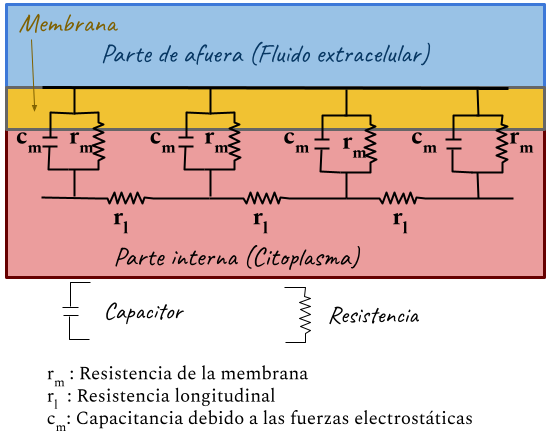
\includegraphics[scale=0.5]{../Figuras/ModeloHH.2}
 \caption{Un primer modelo de la membrana axónica modelada como circuito eléctrico.}
 \label{fig:ModelHh}
\end{figure}

El comportamiento de estas resistencias viene acompañado con un voltaje de reposo, en estos voltajes particulares el tipo de ion (de la resistencia modelada) se estabiliza y ya no va a cambiar esta resistencia. 
Lo que observan es que el ion de sodio y su resistencia va a variar dependiendo del voltaje, a esto se le llama un canal transitorio porque en ciertos voltajes si puede pasar, si es muy bajo, no puede pasar y si rebasa un cierto umbral entonces se vuelve a tapar y ya no puede pasar. 
Lo que sucede con el potasio es que, puede salir si el voltaje está más allá de un cierto valor, si no, no pasan y va variando un poquito que tanto puede pasar. Por estas características de que el potasio es un intervalo dentro de la recta y el sodio es a partir de cierto valor, por tanto se les modelan de maneras ligeramente diferentes. Más adelante se descubrió porque tenían este comportamiento, básicamente el canal de potasio es una puerta hecha de cuatro subpuertas por donde los elementos pasan o no pasan, el canal de sodio es como una compuerta que está hecha de tres subpuertas que se pueden abrir y tiene aparte un tapón extra, que hace que  aunque estas tres están abiertas bloquee toda la compuerta.
 las neuronas están trabajando con muchos más iones aparte de estos dos uno que destaca bastante es el caso del cloro que tiene carga negativa y bueno también se agregó este otro 
 
 elemento que es un canal que está abriendo y cerrando aleatoriamente y está dejando pasar algunos otros iones y eso también va a afectar a la dinámica de la neurona.

entonces con lo que ellos me dieron establecieron me dieron experimentalmente cómo se estaban comportando estas resistencias dependiendo del voltaje del voltaje o la diferencia de potencial que había entre ambos lados de la membrana y a partir de ahí pudieron describir matemáticamente y simular los disparos que se conocen como potenciales de acción 
vamos a mencionar entonces rápidamente cuáles fueron estos conceptos de electricidad que se están utilizando para el modelo tenemos este concepto de 


potenciales eléctricos lo vamos a representar con las letras v dependiendo favorita vamos a ver de lo que más nos convenga y resulten de la separación de cargas opuestas es decir aquí usualmente lo que está sucediendo es que hay mucho sodio acá afuera tres bolitas de sodio que son cargas positiva por dos bolitas de potasio que hay en la parte de adentro entonces hay muchas más cargas positivas en la parte de afuera que las que hay en la parte de adentro y eso es lo que provoca precisamente la diferencia de cargas que es lo que estamos viendo como un este potencial eléctrico estos se van a medir en mil volts el otro elemento son las corrientes movimiento de cargas y se miden en micro amd pers ahora aquí hay una historia es bastante simpática la forma en que hicieron el experimento con el calamar es que literalmente le estaban dando toques al axón entonces lo que hacían ellos era inyectar una corriente eléctrica y gracias a eso lograban ir midiendo que era lo que estaba pasando con las concentraciones de cargas afuera y adentro en el caso de las neuronas reales lo que va a provocar esas cargas esos toques que les daban al ojo quien hizo clic es cuando entran en juego los neurotransmisores y provocan que haya cambios precisamente en estas corrientes entonces digamos que hodgkin y huxley  jugaron el rol que tendrían que jugar usualmente los neurotransmisores para abrir otras compuertas . nosotros en la manera en la que lo vamos a simular es precisamente con estas corrientes que son las que se están poniendo en el experimento y vamos a ver cómo reacciona el acciona 

el otro concepto bueno ya lo estuvimos mencionando la resistencia que es la medida de la oposición en el movimiento de las partículas cargadas 

su inverso matemático es la conductancia es 1 entre r y lo vamos a interpretar como la facilidad de transmisión de las partículas cargadas 

el otro concepto es la capacidad o capacidad eléctrica o capacitancia sé que es la que estamos utilizando aquí para modelar precisamente la membrana estos son lípidos es una grasa es una capita de grasa y esa es la cantidad de energía eléctrica almacenada en un capacitor para una diferencia de potencial eléctrico dada y éste tiene un comportamiento bastante interesante porque las cargas quedan almacenadas un ratito pero se van liberando poco a poco y se va descargando ese capacitor 

\section{Potenciales de Nerst o de reposo}
bueno aquí vemos precisamente porque estamos utilizando la ub y la en la ub generalmente la vamos a utilizar para referirnos a la diferencia de potencial entre la parte de afuera de la célula y la parte de adentro -las es las vamos a utilizar para representar a aquellos voltajes donde cada una de las compuertas encontraría su equilibrio . y como les acababa de mencionar esos voltajes son distintos para cada una de las compuertas esto va a provocar precisamente la dinámica de la de la neurona por ejemplo 

1. aquí vemos que el sodio va a andar cerca de los 50 mil volts ahí estaría su equilibrio es un valor positivo 
2. el calcio que es el que va a jugar un rol ahí aunque se activen los mejores transmisores y se transmita el disparo etcétera etcétera va a estar por ahí de los 150 mil volts o sea que observamos que el voltaje tendría que ser bastante positivo 
3. el potasio que es el que usualmente está trabajando intercambiándose casi todo el tiempo en la neurona va andar por ahí de los menos 80 milvolts de hecho veremos que el punto de equilibrio usual de la neurona anda por el de los menos 76 y 
4. el del cloro está en menos 60 mil volts pues ahí nos podemos pensar que cada uno de estos canales pues está tratando de jalar la dinámica hacia su potencial de equilibrio y bueno no hay precisamente acuerdo entre ellos y eso es precisamente lo que hace que las neuronas cobren vida

\section{Modelo de la membrana como bicapa de lípidos}
\section{Modelo de las compuertas iónicas controladas por voltaje}
\section{Dinámica del voltaje durante un disparo} 
\section{Simulación usando el método de Euler}
\section{Información condificada en las dendritas}

